\documentclass[a4paper,10pt]{ltjsarticle}

% プリアンブル
\usepackage[dvipdfmx]{graphicx}
\usepackage{color}
\usepackage{amsthm}
\usepackage{amsmath}
\usepackage{amsfonts}
\usepackage{mathtools}
\usepackage{listings}
\usepackage[dvipdfmx]{hyperref}
\usepackage{here}
\usepackage{amssymb}
\usepackage{algorithmic}
\usepackage{algorithm}
\usepackage{bbm}
\usepackage{caption}
\usepackage{fancyhdr}
\pagestyle{fancy}
\lhead{Survey by D. Nishiyama on \today}    % ヘッダの右側
%\cfoot{\thepage}                % フッター中央
\renewcommand{\headrulewidth}{0pt}        % ヘッダの線の太さ:0ptで消える

\newcommand{\bi}[1]{\ensuremath{\boldsymbol{#1}}}
\newcommand{\propose}{Class-Sensitive}
\newcommand{\multicell}[2]{\begin{tabular}{c}
                               #1\\#2
\end{tabular}}


% 転置記号
\newcommand{\T}{\ensuremath{^{\text{T}}}}

% 図の参照
\newcommand{\Zu}[1]{図\ref{fig:#1}}

% 表の参照
\newcommand{\Hyou}[1]{表\ref{tab:#1}}
\newcommand{\II}{I\hspace{-.1em}I}
% 式の参照
\newcommand{\Shiki}[1]{式\eqref{eq:#1}}
\newcommand{\1}{\mbox{1}\hspace{-0.25em}\mbox{l}}
\lstset{
    basicstyle={\ttfamily\small}, %書体の指定
    frame=tRBl, %フレームの指定
    framesep=10pt, %フレームと中身(コード)の間隔
    breaklines=true, %行が長くなった場合の改行
    linewidth=15cm, %フレームの横幅
    lineskip=-0.5ex, %行間の調整
    tabsize=2 %Tabを何文字幅にするかの指定
}
\usepackage{multirow}
\usepackage{stmaryrd}
\usepackage{subfiles}
\theoremstyle{definition}
\newtheorem{theorem}{定理}
\newtheorem*{theorem*}{定理}
\newtheorem{prop}{命題}
\newtheorem*{prop*}{命題}
\newtheorem{definition}[theorem]{定義}
\newtheorem*{definition*}{定義}

\def\hlineb{%
    \noalign{\ifnum0=`}\fi\hrule \@height \arrayrulewidthb \futurelet
    \reserved@a\@xhlineb}
\def\@xhlineb{\ifx\reserved@a\hlineb
\vskip\doublerulesep
\vskip-\arrayrulewidthb
\fi
\ifnum0=`{\fi}}

\newcommand{\argmax}{\mathop{\rm arg~max}\limits}
\newcommand{\argmin}{\mathop{\rm arg~min}\limits}
\title{Explainability in Graph Neural Networks: An Experimental Survey\cite{georgiev2021algorithmic}}
\author{Peibo Li , Yixing Yang , Maurice Pagnucco and Yang Song}
\date{17 Mar 2022, Under review}

%!  心構え
%!  ・時間を決めて読む
%!  ・まとめる癖をつける


%! 読む順番 パターンA(じっくり)
%!  1.アブストラクト(何をしたか)、イントロダクション(何をしたいか)
%!  2.結論(何をしたか・詳細)
%!  3.実験結果(主張の証明)・議論(良し悪し)
%!  4.関連研究(他との違い)、メソッド(実験方法)

%! 読む順番 パターンB(ざっくり)
%!  1.アブストラクト(何をしたか)
%!  2.イントロダクション(何をしたいか)
%!  3.結果(主として図)
% Document
\begin{document}
    \maketitle
    \abstract{グラフニューラルネットワーク(GNN)モデルに関する最近の研究では、古典的なグラフアルゴリズムや組合せ最適化問題へのGNNの適用に成功した。これには、前提条件が満たされない場合のアルゴリズムの適用や、十分な学習データが得られない、あるいは生成できない場合の学習済みモデルの再利用など、数多くの利点があります。しかし、GNNはブラックボックスモデルであり、直接解釈することができないため、これらのアプローチの主な障害は、説明可能性に欠けることである。本研究では、概念に基づく説明に関する既存の研究をGNNモデルに適用することで、この制限を解決する。GNNの読み出し機構を修正した概念ボトルネックGNNを導入する。3つのケーススタディを用いて、我々は以下のことを実証する。(i)提案モデルが、各ターゲットクラスに対して、正確に概念を学習し、学習した概念に基づく命題式を抽出できること、(ii)提案概念ベースGNNモデルが、最先端モデルとの比較性能を達成できること、(iii)グラフレベルの概念に対して明示的にスーパービジョンを与えずに、グローバルグラフ概念を導出できること、である。}

    concept: 概念

    !イントロの書き方が自分の研究の参考になりそう


    \section{どういう論文?}
    conclusionから
    \begin{itemize}
        \item グラフアルゴリズムにおける概念に基づく推論機構を持つConcept Bottleneck Graph Neural Networksを提案
        \item これを通して、性能に影響を与えることなく、ノードレベルの概念を正確に学習できることを示した
        \item 学習データとモデルの重みを調べることで、定義された概念に基づき、各ノードレベルの出力クラスを数式で説明することが可能である
        \item 概念によって、特定のグラフレベルのタスク(終了時期の決定など)の教師なしルール抽出を行うことができる
        \item 抽出されたルールは解釈可能であり、ルールを適用しても精度に大きな影響を与えない
    \end{itemize}
    \begin{figure}[H]
        \centering
        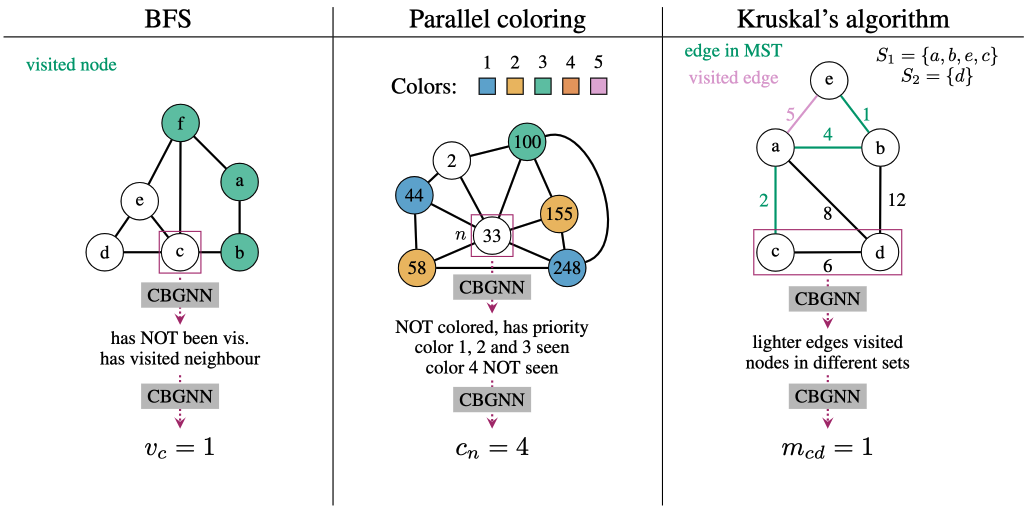
\includegraphics[width=120mm]{fig/cbgnn_1}
        \caption{概念ボトルネックグラフニューラルネットワーク(CBGNN)アプローチの概要。重要なことは、CBGNNモデルは、アルゴリズムのルールだけでなく、与えられたタスクのための概念情報を抽出するために訓練することができることです。3つのアルゴリズムの例を挙げ、CBGNNがどのように入力データから概念を抽出し、それを使って出力をどのように計算するのかを示す。}
    \end{figure}


    \section{先行研究と比べてどこがすごい?}
    GNN Explainability
    \begin{itemize}
        \item 既存法:
        \begin{itemize}
            \item \cite{pope2019explainability, baldassarre2019explainability, schnake2020higher}の研究は、
            個々の予測を担う最も重要なノード/サブグラフを特定するために、CNNアプリケーションに用いられる特徴重要度勾配ベースのアプローチ
            (Class Activation MappingsやLayer-wise Relevance Propagationなど)をGNNsに適応
            \item \cite{ying2019gnnexplainer, vu2020pgm, luo2020parameterized}の研究は、
            相互情報量の最大化に基づくものや、特徴説明のマルコフブランケット条件付き確率など、GNN説明可能性に特有の、より複雑なアプローチに焦点を当てている
        \end{itemize}
        これらの研究は、
        \begin{itemize}
            \item 本研究の焦点である組み合わせ最適化タスクに焦点を当てるのではなく、ソーシャルネットワーク、化学、または創薬に関わるGNNタスクとベンチマークに焦点を当てていることである。
            \item 事前に訓練されたGNNを事後的に説明することに焦点を当てている
            \item 特徴量に基づく説明アプローチ(すなわち、入力ノード/サブグラフの相対的重要性を保持すること)に焦点を当てている
        \end{itemize}
        \item 我々は、解釈可能なGNNモデルを構築することに焦点を当てている。
        \item 我々は代わりに概念に基づく説明アプローチに依存している。
    \end{itemize}

    Concept-based Explainability
    \begin{itemize}
        \item 既存のconcept baseの説明手法ははCNNの文脈でのみ概念を探求している
        \item RNNモデルの文脈で概念を探求している研究は\cite{kazhdan2020meme}だけであることである
        \item この研究では、GNNのための概念に基づく説明可能性に焦点を当て、\cite{koh2020concept}と同様に、概念は人間が指定したものとする
    \end{itemize}

    Combinatorial Optimisation for GNNs
    \begin{itemize}
        \item 提案法は\cite{velivckovic2020pointer, velivckovic2019neural}の拡張
        \item \cite{velivckovic2020pointer}だけが\cite{ying2019gnnexplainer}で説明を試みている
        \item しかし、彼らのモデルは、
        \begin{enumerate}
            \item モデル構造による説明可能性がなく
            \item 局所的な説明を与えるために、単一のサンプルに対してさらなる最適化を必要とした。
        \end{enumerate}
        \item 他のすべての先行研究はブラックボックス方式で動作し、学習されたモデルの説明可能性を考慮しなかった。
    \end{itemize}


    \section{技術や方法のポイントはどこ?}
    \begin{itemize}
        \item GNNモデルの出力の前にコンセプトボトルネック層を適用する
        \item 中間概念処理に依存した新しいタイプのGNNである概念ボトルネックグラフニューラルネットワーク(CBGNN)を提案する。本論文は、概念ボトルネック法をGNNに適用した最初の研究である。
        \item 適切な概念の集合に依存し、それを監督することで、幅優先探索、クラスカルのアルゴリズムなどの古典的アルゴリズムのルールや、並列グラフコーディングなどのより進んだヒューリスティクスを導くことができること
    \end{itemize}
    \begin{figure}[H]
        \centering
        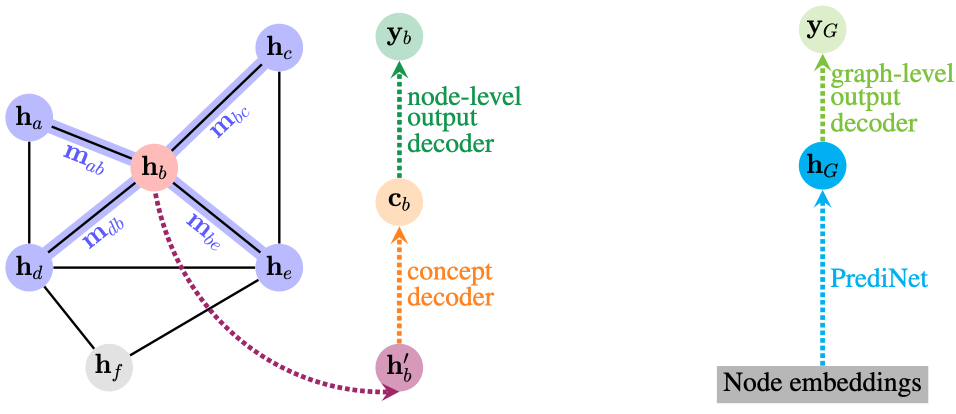
\includegraphics[width=120mm]{fig/cbgnn_2}
        \caption{左:ノードレベルの出力を生成するために、隣接ノードからのメッセージ$m_{ij}$は
        現在のノード表現$h_b$と結合され、結果として更新された表現$h^\prime_b$となる。
        右:ノード埋め込みをPrediNetに通すことで、グラフレベルの埋め込み$h_G$を得ることができる。
        グラフレベルの出力$y_G$(ここでは終了確率)を潜在状態$h_G$から直接抽出する。
        グラフレベルの概念は、ノード概念に対する完全な列挙アプローチにより抽出される。}
    \end{figure}
    \begin{equation}
        \begin{aligned}
            \mathbf{z}_{i}^{(t)} &=f_{A}\left(\mathbf{x}_{i}^{(t)}, \mathbf{h}_{i}^{(t-1)}\right) \\
            \mathbf{z}_{i}^{\prime(t)} &=f_{A}\left(\mathbf{y}_{i}^{(t)}, \mathbf{h}_{i}^{(t)}\right) \\
            \mathbf{H}^{(t)} &=P\left(\mathbf{Z}^{(t)}, E\right) \\
            \mathbf{H}^{\prime(t)} &=P\left(\mathbf{Z}^{\prime(t)}, E\right) \\
            \mathbf{c}_{i}^{(t)} &=\sigma\left(g_{A}^{\prime}\left(\mathbf{z}_{i}^{(t)}, \mathbf{h}_{i}^{(t)}\right)\right) \\
            \overline{\mathbf{H}^{(t)}} &=\operatorname{PrediNet}\left(\mathbf{H}^{\prime}(t)\right.\\
            \mathbf{y}_{i}^{(t)} &=g_{A}\left(\mathbf{c}_{i}^{(t)}\right) \\
            \tau^{(t)} &=\sigma\left(T_{A}\left(\overline{\mathbf{H}^{(t)}}\right)\right)
        \end{aligned}
    \end{equation}
    where $\sigma$ is a logistic sigmoid function.


    \section{どうやって有効と検証した?}
    \begin{itemize}
        \item 3種類のケーススタディ(BFS、グラフカラー化、クラスカール)を用いて本アプローチを定量的に評価し、CBGNNアプローチが既存の最先端技術と同等の性能を達成できることを示す。
        \item CBGNNモデルによって利用される概念が、CBGNNが学習したヒューリスティックを要約するルールを提供するためにどのように利用できるかを示すことによって、我々のアプローチを定性的に評価する。
    \end{itemize}


    \section{議論はある?}
    \begin{itemize}
        \item GNNはこれらのアルゴリズム課題に対して、ノードまたは近傍情報を含む高レベルの概念を生成することができ、学習された概念抽出器は強く汎化されることがわかる(5倍大きいグラフに対しても概念の精度は落ちない)。
        \item ボトルネックは最終的なモデルの精度に大きな影響を与えない
    \end{itemize}


    \section{次に読むべき論文は?}

    \bibliographystyle{apalike}
    \bibliography{/Users/funami/Documents/Survey/ref}
\end{document}


